Hier werden die Netze jeweils einmal mit und einmal ohne Transferlernen ausgetestet. Es werden nur die Direct Cascade Netzwerke betrachtet und 
sie werden mit deutlich mehr Netziterationen trainiert als bisher. Die Epochenanzahl pro Netzwerk bleibt aber gleich. Dabei werden jeweils nur 
wenig Targetdaten verwendet. 

\begin{figure}[htpb]
    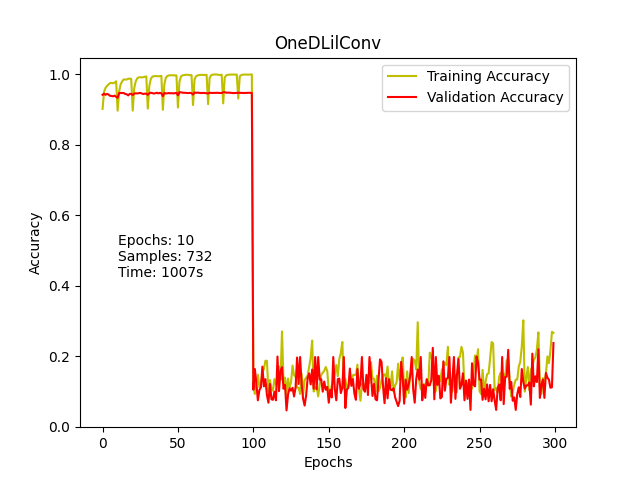
\includegraphics[height=5cm]{../../Plots/ba_plots/classTF/1dc_tr.png}
    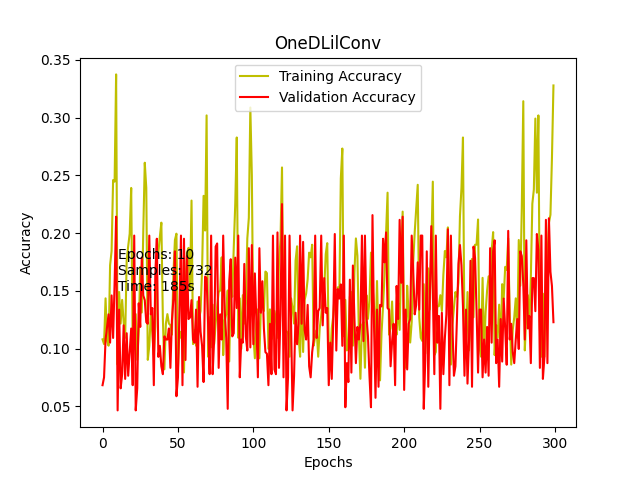
\includegraphics[height=5cm]{../../Plots/ba_plots/classTF/wo1dc_tr.png}
    \caption{\label{fig:1dc_tr} 1DConv TF Vergleich}
\end{figure}

Wie in Figure 4.4 zu sehen gibt es keinen Unterschied zwischen der Accuracy mit TF zu der ohne bei Convolutionlayern. In beiden Fällen ist diese 
extrem schlecht. Dies zeigt sich auch auf den Testdaten. 

\begin{figure}[htpb]
    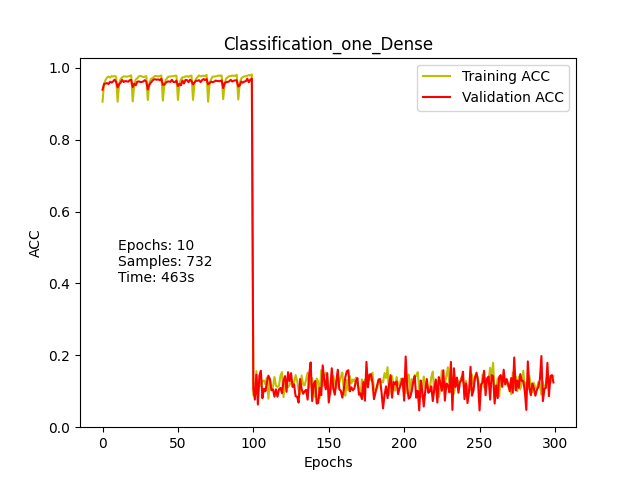
\includegraphics[height=5cm]{../../Plots/ba_plots/classTF/cod_tr.png}
    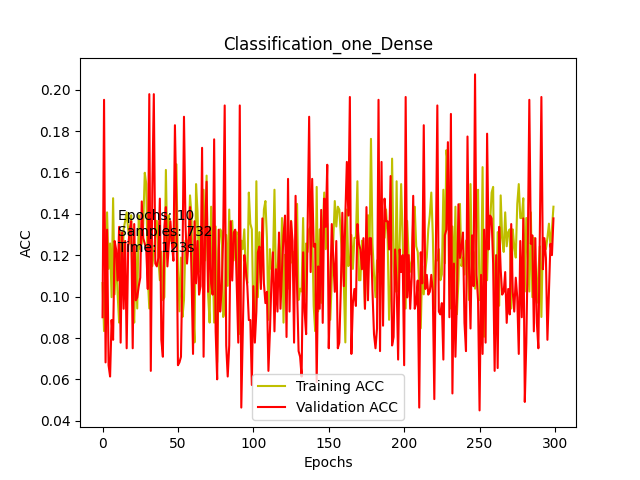
\includegraphics[height=5cm]{../../Plots/ba_plots/classTF/wocod_tr.png}
    \caption{\label{fig:cod_tr} ClassOneDense TF Vergleich}
\end{figure}

In Figure 4.5 zeigt sich dasselbe Bild nur auf Basis von Linearlayern. Dies kann zwei Gründe haben: Entweder funktioniert das Kaskadieren nicht 
oder es sind nicht genügend Targetdaten vorhanden. Letzteres wurde oben ausgetestet und lieferte zwar bessere, aber trotzdem nur mäßige Ergebnisse. 
